\documentclass[a4paper, 14pt]{extarticle}
\usepackage{enumitem}
\usepackage{fefutitle}
\usepackage{xcolor}
\usepackage{amsmath}
\usepackage{graphicx}
\usepackage[justification=centering]{caption}
\usepackage{float}

\begin{document}
	\fefutitle{6}{Задача переноса примесей}
	\pagebreak	

	\section{Введение}
		В данной лабораторной работе необходимо создать модель переноса примесей. В качестве объекта для создания модели возьмем закрытую акваторию с заданным полем концентрации в начальный момент времени и стационарным полем скорости. Необходимо определить поле концентрации в любой момент времени в стационарном поле скорости.
	\section{Создание математической модели}
	 	Для моделирования процессов распространения используется уравнение переноса. Уравнение переноса -- дифференциальное уравнение в частных производных, описывающее изменение скалярной величины в пространстве.
		Уравнение переноса имеет следующий вид:
		\[\dfrac{\partial C}{\partial t} + u \dfrac{\partial C}{\partial x} + \upsilon \dfrac{\partial C}{\partial y} = 0 \], где $t$ - время, $C$ - концетрация, $x$ и $y$ - координаты, $u$ - компонента скорости на $x$, $\upsilon$ - компонента скорости на $y$.
		
		В начальный момент задано поле концетрации:
		\[ C(x, y, t) = C0(x, y)\]
		
		Концентрация точек будет постоянной и не меняться со временем
		
		\bigg($\dfrac{dC}{dt} = 0$\bigg).
		
		Поле скорости зададим через функцию тока $\psi = \psi(x, y)$ с компонентами скорости:
		\[ \begin{cases}
			u (x, y) = -\dfrac{\partial \psi}{\partial y} \\[7pt]
			\upsilon (x, y) = \phantom{-} \dfrac{\partial \psi}{\partial x}
		\end{cases} \]
		
		Для численного решения уравнений в частных производных существует несколько способов. Один из них, который будет использоваться в данной лабораторной работе -- метод частиц. Метод частиц состоит в представлении тела совокупностью взаимодействующих частиц(материальных точек), описываемых законами классической механики.
		Составим систему дифференциальных уравнений для каждой частицы:
		\[ \begin{cases}
				\dfrac{dx_i}{dt} = u(x_i, y_i), \\[7pt]
				\dfrac{dy_i}{dt} = \upsilon(x_i, y_i)
			\end{cases}
		\]

	\section{Реализация модели}	
		Для модели создадим $20$ тысяч частиц с начальными координатами от 0 до 1.
		
		За поле скорости возьмем следующую функцию тока:
		\[ \psi = \sin(2\pi x) \cdot \sin(\pi y) \]
		
		с компонентами скорости:
		\[ \begin{cases}
			u (x, y) = -\pi \cdot \sin{(2\pi x)} \cdot \cos{(2\pi)} \\[7pt]
			\upsilon (x, y) = 2\pi \cdot \cos{(2\pi x)} \cdot \sin{(\pi y)} 
		\end{cases} \]
		
		\begin{figure}[H]
			\centering
			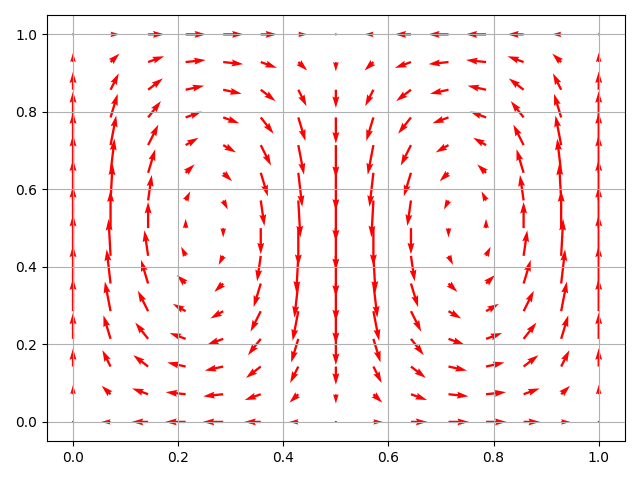
\includegraphics[width = .5\linewidth]{11.png}
			\caption[.] {Функция тока $\psi = \sin(2\pi x) \cdot \sin(\pi y)$}
		\end{figure}
		
		Для каждой частицы зададим начальную концентрацию:
		\[ C0(x, y) = \arctan{\Bigg(\dfrac{y-0.5}{0.1}\Bigg)} \]
			
		Модель была реализована в Python. Для решения системы дифференциальных уравнений используется функция odeint, которая численно решает её методом Рунге-Кутты 4 порядка. Она принимает 3 параметра: система дифференциальных уравнений, начальные значения и интервал, на котором строится решение. Для интерполяции на прямоугольную сетку с помощью билинейной интерполяции используется функция griddata. Она принимает координаты точек, значения в них и сетку, на которую будет интепорлировать.
		\begin{figure}[H]
			\begin{minipage}{0.5\textwidth}
				\centering
				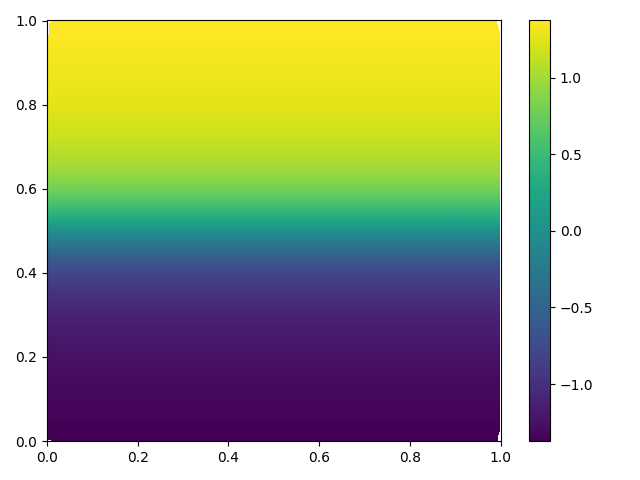
\includegraphics[width = \linewidth]{1.png}
			\end{minipage}\hfill
			\begin{minipage}{0.5\textwidth}
				\centering
				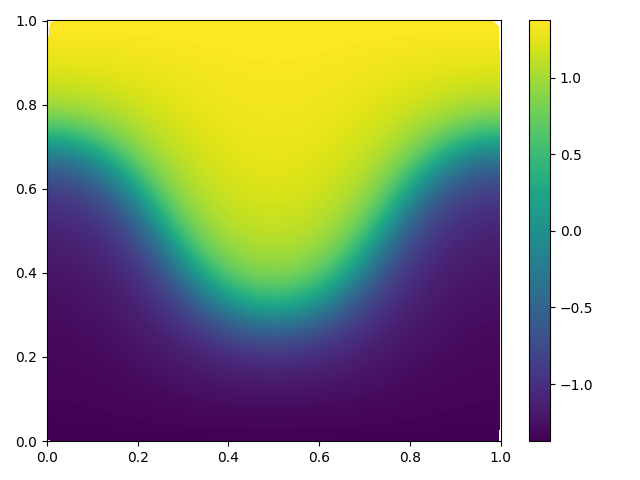
\includegraphics[width = \linewidth]{2.png}
			\end{minipage}\hfill
		\end{figure}
	
		\begin{figure}[H]
			\begin{minipage}{0.5\textwidth}
				\centering
				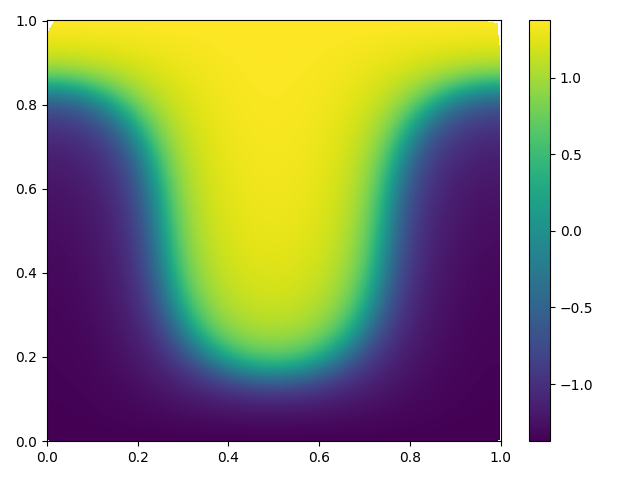
\includegraphics[width = \linewidth]{3.png}
			\end{minipage}\hfill
			\begin{minipage}{0.5\textwidth}
				\centering
				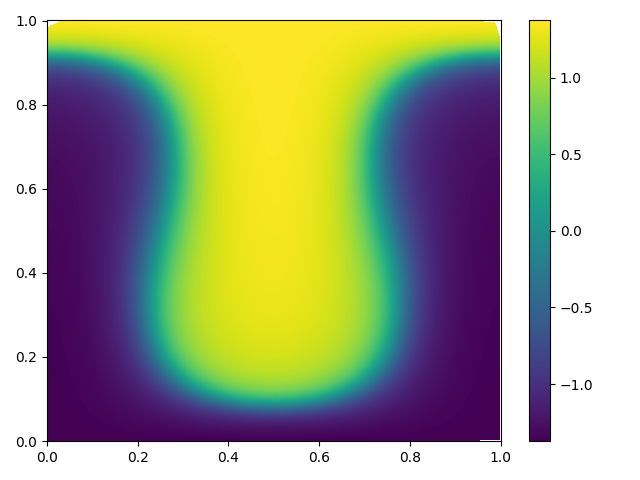
\includegraphics[width = \linewidth]{4.png}
			\end{minipage}\hfill
		\end{figure}
	
		\begin{figure}[H]
			\begin{minipage}{0.5\textwidth}
				\centering
				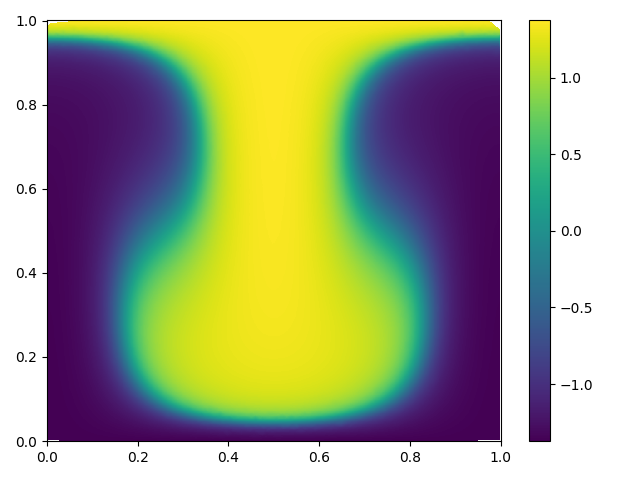
\includegraphics[width = \linewidth]{5.png}
			\end{minipage}\hfill
			\begin{minipage}{0.5\textwidth}
				\centering
				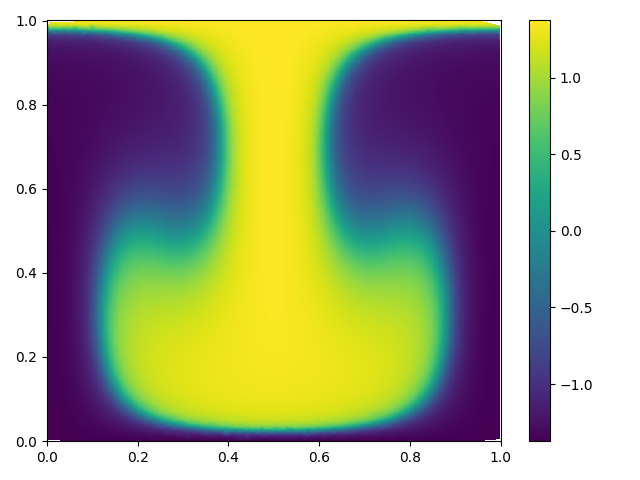
\includegraphics[width = \linewidth]{6.png}
			\end{minipage}\hfill
		\end{figure}
	
		\begin{figure}[H]
			\begin{minipage}{0.5\textwidth}
				\centering
				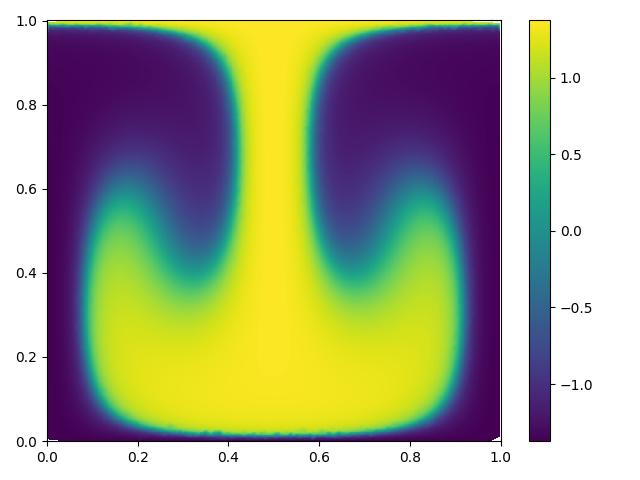
\includegraphics[width = \linewidth]{7.png}
			\end{minipage}\hfill
			\begin{minipage}{0.5\textwidth}
				\centering
				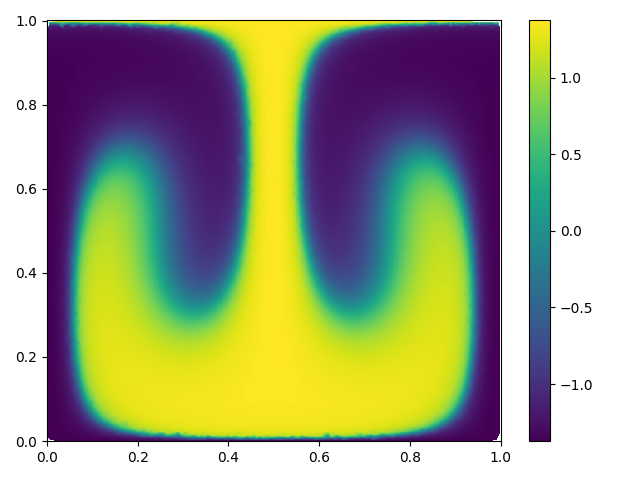
\includegraphics[width = \linewidth]{8.png}
			\end{minipage}\hfill
		\end{figure}
	
		\begin{figure}[H]
			\begin{minipage}{0.5\textwidth}
				\centering
				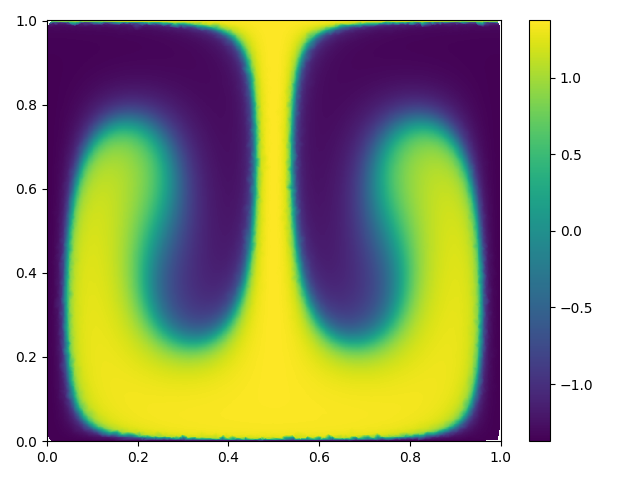
\includegraphics[width = \linewidth]{9.png}
			\end{minipage}\hfill
			\begin{minipage}{0.5\textwidth}
				\centering
				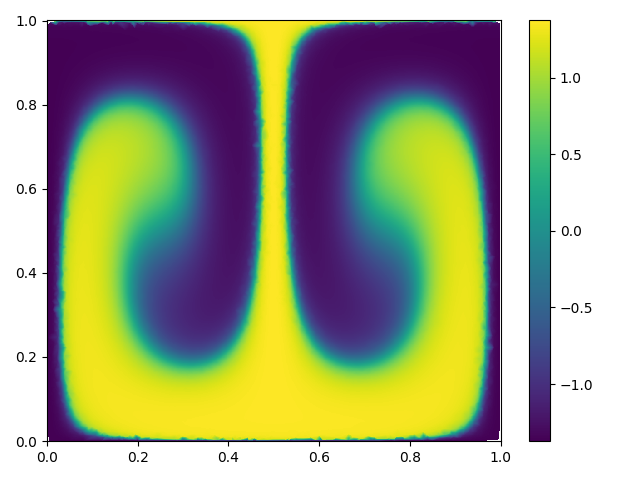
\includegraphics[width = \linewidth]{10.png}
			\end{minipage}\hfill
		\end{figure}
		
	\section{Заключение}
		В ходе лабораторной работы была создана и реализована модель переноса примесей в стационарном поле скорости.
\end{document}	